\chapter[Resultados Obtidos]{Resultados Obtidos}

O principal problema encontrado na execução da atividade foi a questão da persistência dos
dados. Isso acontecia quando determinado elemento era inserido e, por coincidência, esse mesmo
elemento já se encontrava em uma fila diferente. A medida que novos elementos eram inseridos as referências dos elementos enfileirados eram perdidas.

Um fator que gerou uma quantidade considerável de trabalho manual e, por isso, demandou um grande período de tempo, foi a questão da inserção dos dados referentes às distâncias entre cidades dentro dos arquivos de
texto. Não se tratava de uma tarefa de difícil abstração, porém trabalhou-se com muitos arquivos com campos
a serem estudados.

Outro ponto que causou certa dificuldade foi o fato de se tratar da primeira experiência usando grafos,
que é um assunto fora do escopo da disciplina exigindo portanto vários estudos complementares para
fundamentação dos conceitos.

A escolha do paradigma Orientado a Objetos na resolução do problema poderia gerar \textit{overhead}, mas essa decisão se mostrou acertada uma vez que essa abordagem abriu um leque de novas funcionalidades e
formas de trabalhar que, caso usadas de maneira correta, facilitariam a realização da solução.

Durante a execução do trabalho não foi possível encontrar problemas decorrentes da falta de recursos
computacionais e nem de estouro de memória, o que demonstra que se atingiu uma solução de
grande qualidade. Outro ponto que deve ser destacado é que as respostas são apresentadas de forma instantânea à inserção das entradas, independente de se tratar de casos muito complexos ou não. Deve-se levar em consideração que o desenvolvimento foi executado e testado em plataformas Linux com mais de 4 GB de \textit{ram}.

\section{Descrição da Performance}

\begin{figure}[!htb]
 \centering
 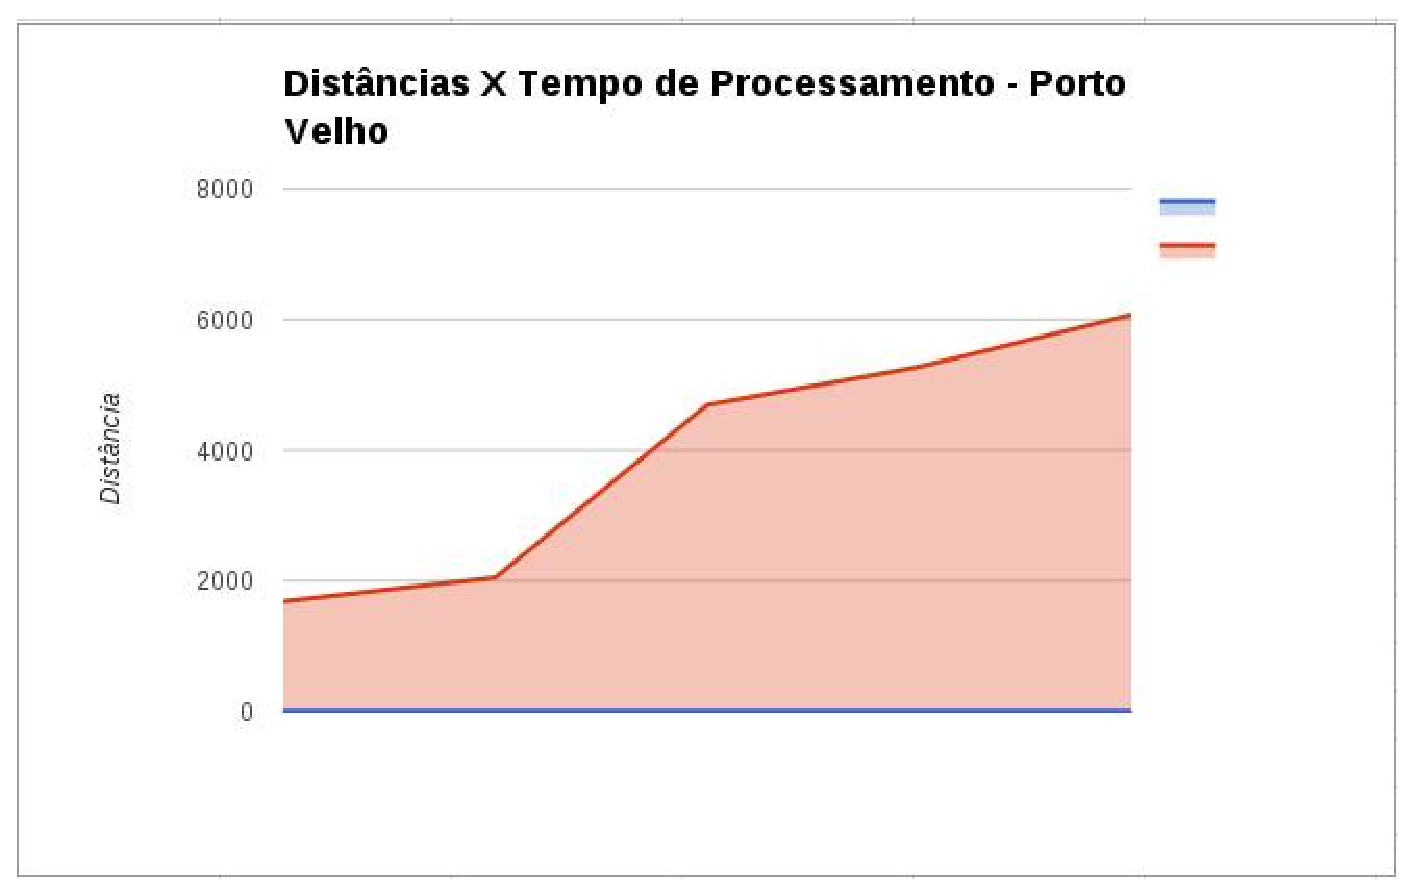
\includegraphics[scale= 0.3]{figuras/imagem1.eps}
 \caption{Gráfico referente a capital Porto Velho.}
\end{figure}

\begin{figure}[!htb]
 \centering
 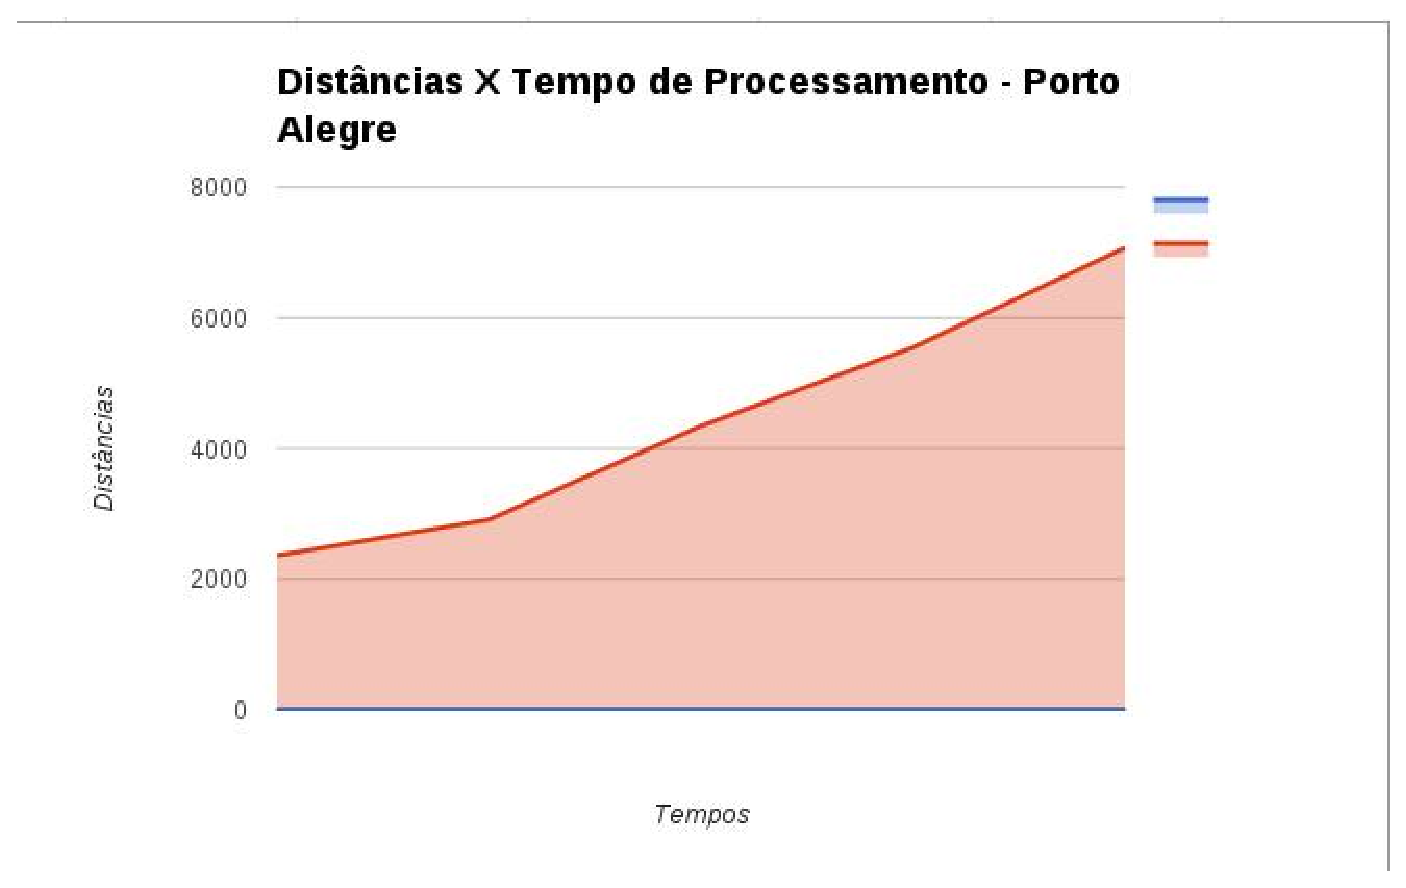
\includegraphics[scale= 0.3]{figuras/imagem2.eps}
 \caption{Gráfico referente a capital Porto Alegre.}
\end{figure}

\begin{figure}[!htb]
 \centering
 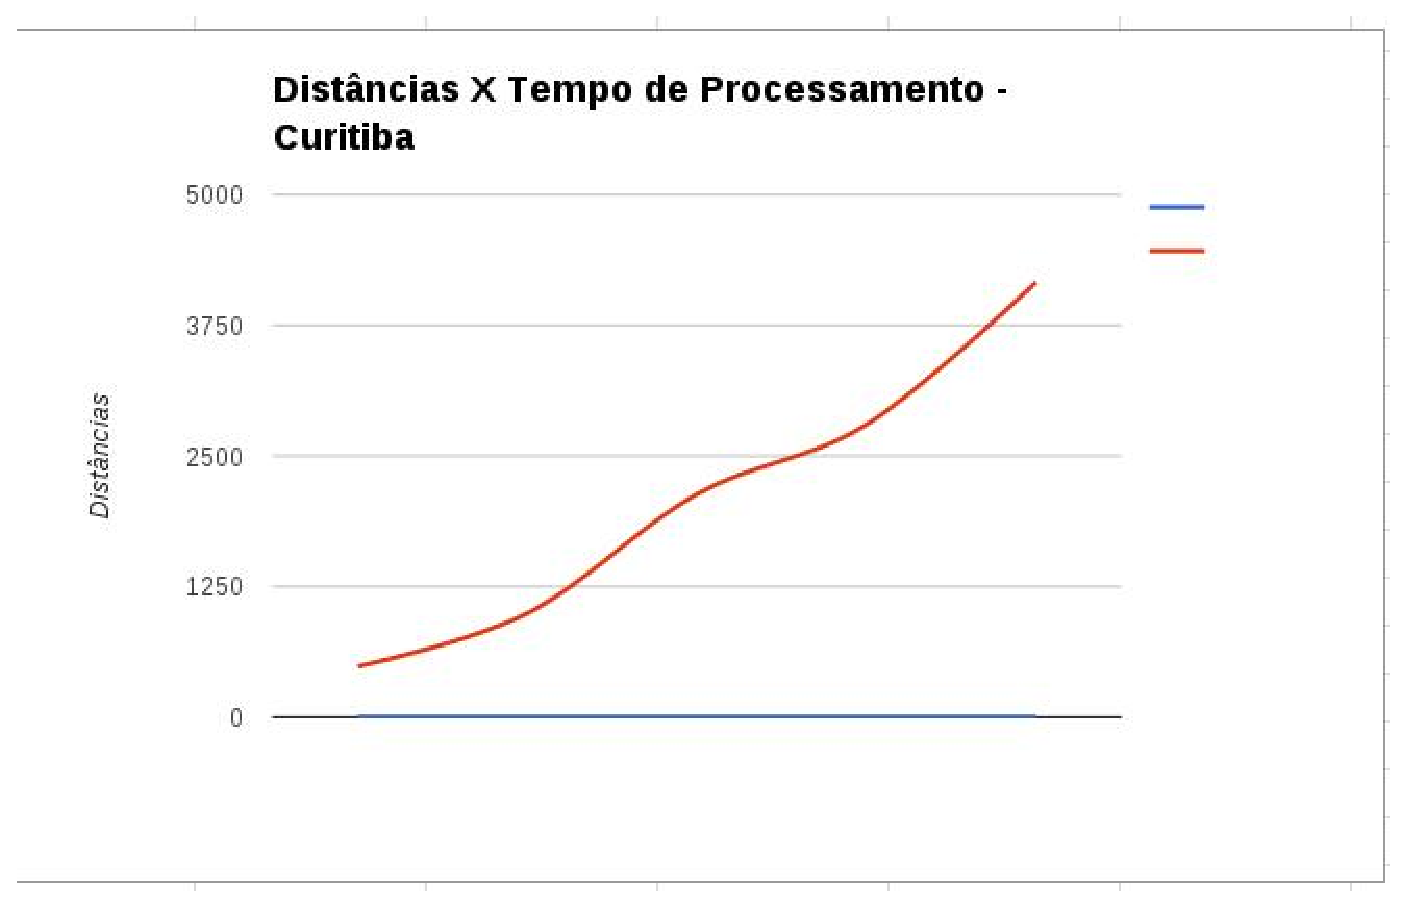
\includegraphics[scale= 0.3]{figuras/imagem3.eps}
 \caption{Gráfico referente a capital Curitiba.}
\end{figure}

\begin{figure}[!htb]
 \centering
 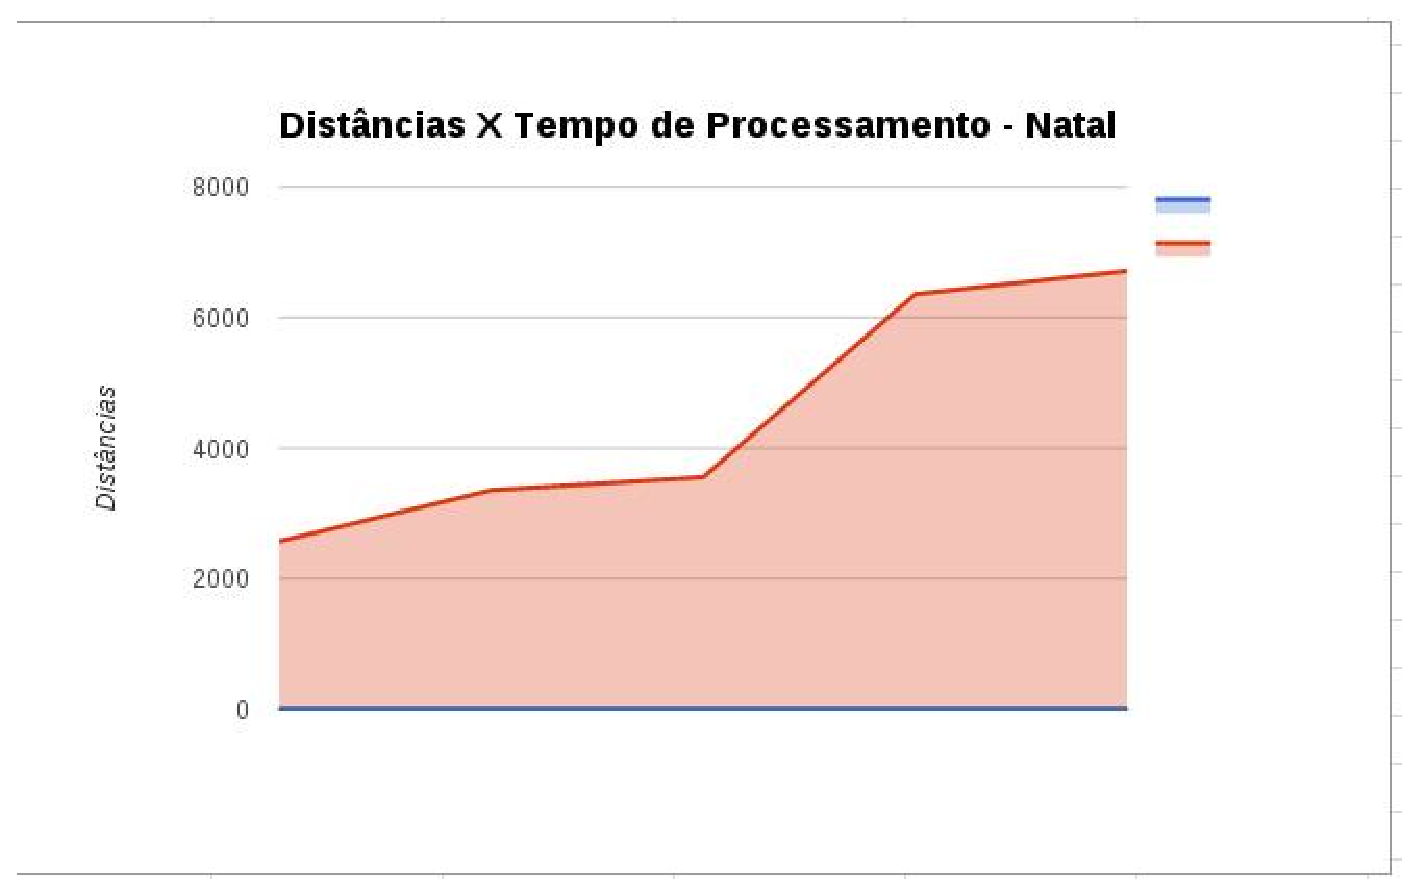
\includegraphics[scale= 0.3]{figuras/imagem4.eps}
 \caption{Gráfico referente a capital Natal.}
\end{figure}